\documentclass[11pt, a4paper, bold, center, twoside, journal]{paper}

\usepackage[bottom = 2.5cm, top = 2.5cm, inner= 2cm, outer = 1.5cm]{geometry}

\usepackage[utf8]{inputenc} 
\usepackage[T5]{fontenc} 
\usepackage[vietnamese]{babel}
 
\usepackage{amssymb, amsthm}
\usepackage[intlimits]{mathtools}
\usepackage{graphicx}

\usepackage{float}%*\label{line:baibao_standalone_dqtuyen_main_float}*)
\usepackage{multicol}%*\label{line:baibao_standalone_dqtuyen_multicol}*)

\def\submit{\small (Nhận ngày:..., Đăng ngày:...)}%*\label{line:baibao_standalone_dqtuyen_submit}*)



\begin{document}

\title{Ứng dụng phổ $\gamma$ trong nghiên cứu cấu trúc hạt nhân $^{156}$Gd}

\author{Đoàn Quang Tuyền\textsuperscript{a}\thanks{email: abc@gmail.com \newline tel: 0912345678}~, Nguyễn Văn A\textsuperscript{a,b}, 
	Nguyễn Văn B\textsuperscript{b}, 
	Nguyễn Văn C\textsuperscript{a}
}
\institution{
	\textsuperscript{a}Viện nghiên cứu hạt nhân\\
	\textsuperscript{b}Đại học khoa học tự nhiên
}

\date{\submit}
\shortauthor{Đoàn Quang Tuyền, Nguyễn Văn A, Nguyễn Văn B, Nguyễn Văn C}
\shorttitle{Ứng dụng phổ $\gamma$ trong nghiên cứu cấu trúc hạt nhân $^{156}$Gd}
\oddrunhead{D. Q. Tuyen et al.}
\evenrunhead{Ứng dụng phổ $\gamma$ trong nghiên cứu cấu trúc hạt nhân $^{156}$Gd}

\maketitle

\begin{abstract}
Tóm tắt nội dung của bài báo, nêu vấn đề, cách giải quyết vấn đề, các kết quả chính và kết luận, kiến nghị. Tóm tắt nội dung của bài báo, nêu vấn đề, cách giải quyết vấn đề, các kết quả chính và kết luận, kiến nghị. Tóm tắt nội dung của bài báo, nêu vấn đề, cách giải quyết vấn đề, các kết quả chính và kết luận, kiến nghị. Tóm tắt nội dung của bài báo, nêu vấn đề, cách giải quyết vấn đề, các kết quả chính và kết luận, kiến nghị ...
\end{abstract}

\begin{keywords}
Cấu trúc hạt nhân, phổ gamma, ghi nhận bức xạ.
\end{keywords}

%%%%%%%%%%%%%%%%%
\begin{multicols}{2}%*\label{line:baibao_standalone_dqtuyen_multicol_use}*)

\section{Mở đầu}

Tiết diện tán xạ\footnote{Tính theo đơn vị bar.} của các tia bức xạ $\gamma$ được thể hiện thông qua phương trình \ref{equ:compton}(xem tài liệu \cite{bib_Klein, bib_Knoll}).  

Trình bày các đoạn văn bản và các công thức toán học hoặc hình vẽ có liên quan tới nội dung của để mục giống như đôi với luận văn, luận án, hoặc các bài báo cáo. Trình bày các đoạn văn bản và các công thức toán học hoặc hình vẽ có liên quan tới nội dung của để mục giống như đôi với luận văn, luận án, hoặc các bài báo cáo. Trình bày các đoạn văn bản và các công thức toán học hoặc hình vẽ có liên quan tới nội dung của để mục giống như đôi với luận văn, luận án, hoặc các bài báo cáo ... 


\end{multicols}%*\label{line:baibao_standalone_dqtuyen_multicol_use_stop}*)

\begin{equation}
\cfrac{d \sigma_{e}}{d \Omega} = \cfrac{r_{0}^{2}}{2} 
\biggl\{
	\cfrac{1}{[1+\alpha(1-cos\theta)]^{2}}
	\biggl [
	1+cos^{2}\theta+\cfrac{\alpha^{2}(1-cos\theta)^{2}} {[1+\alpha(1-cos\theta)]}
	\biggr ]
\biggr\}
\label{equ:compton}
\end{equation}

\vspace{\parskip}
\begin{multicols}{2}%*\label{line:baibao_standalone_dqtuyen_multicol_use_restart}*)

Trình bày các đoạn văn bản và các công thức toán học hoặc hình vẽ có liên quan tới nội dung của để mục giống như đôi với luận văn, luận án, hoặc các bài báo cáo. Trình bày các đoạn văn bản và các công thức toán học hoặc hình vẽ có liên quan tới nội dung của để mục giống như đôi với luận văn, luận án, hoặc các bài báo cáo. Trình bày các đoạn văn bản và các công thức toán học hoặc hình vẽ có liên quan tới nội dung của để mục giống như đôi với luận văn, luận án, hoặc các bài báo cáo ... 

\subsection{Cấu trúc hạt nhân}
Các mức năng lượng của hạt nhân được trình bày trên Hình \ref{fig:nangluong}...

Trình bày các đoạn văn bản và các công thức toán học hoặc hình vẽ có liên quan tới nội dung của để mục giống như đôi với luận văn, luận án, hoặc các bài báo cáo. Trình bày các đoạn văn bản và các công thức toán học hoặc hình vẽ có liên quan tới nội dung của để mục giống như đôi với luận văn, luận án, hoặc các bài báo cáo. Trình bày các đoạn văn bản và các công thức toán học hoặc hình vẽ có liên quan tới nội dung của để mục giống như đôi với luận văn, luận án, hoặc các bài báo cáo ... 

\end{multicols}%*\label{line:baibao_standalone_dqtuyen_multicol_use_stop2}*)

\begin{figure}[!htb]
\centering
	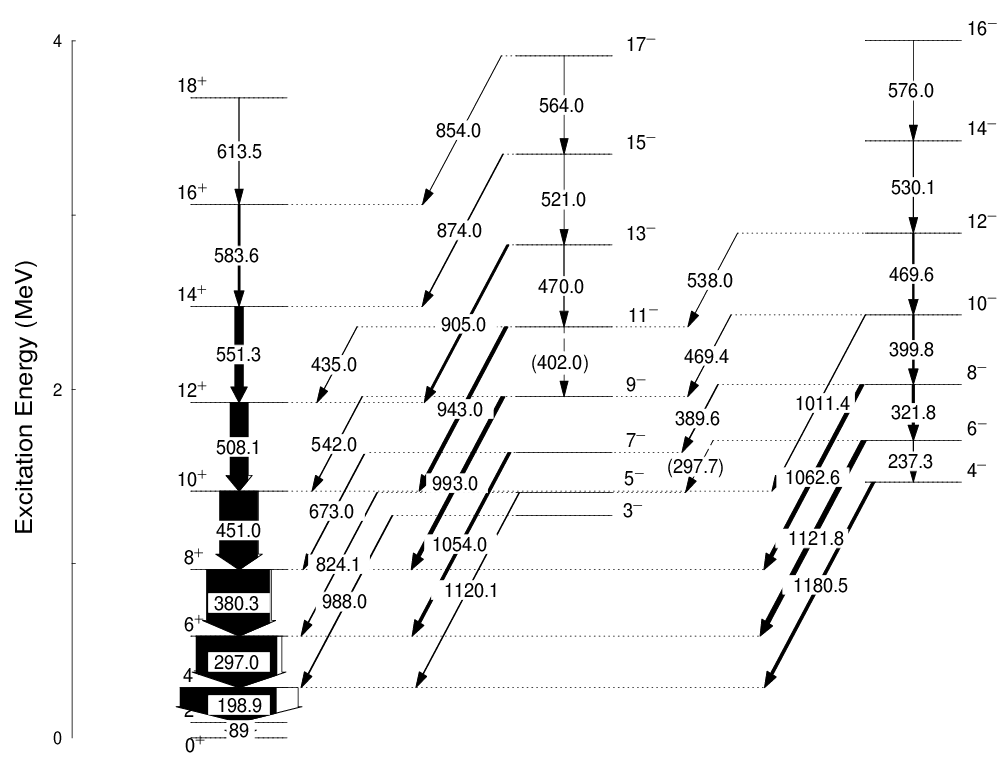
\includegraphics[width=0.4\textwidth]{figure/156Gd.png}
	\caption{Mức năng lượng của hạt nhân.}
	\label{fig:nangluong}
\end{figure}

\begin{multicols}{2}%*\label{line:baibao_standalone_dqtuyen_multicol_use_restart2}*)

Trình bày các đoạn văn bản và các công thức toán học hoặc hình vẽ có liên quan tới nội dung của để mục giống như đôi với luận văn, luận án, hoặc các bài báo cáo. Trình bày các đoạn văn bản và các công thức toán học hoặc hình vẽ có liên quan tới nội dung của để mục giống như đôi với luận văn, luận án, hoặc các bài báo cáo. Trình bày các đoạn văn bản và các công thức toán học hoặc hình vẽ có liên quan tới nội dung của để mục giống như đôi với luận văn, luận án, hoặc các bài báo cáo ... 

\subsection{Phổ $\gamma$}
Các phổ $\gamma$\footnote{Ghi nhận bởi detector} đã được nghiên cứu trong các tài liệu \cite{bib_Bazzaco, bib_Simpson, bib_ghinhanbucxa} ...

Trình bày các đoạn văn bản và các công thức toán học hoặc hình vẽ có liên quan tới nội dung của để mục giống như đôi với luận văn, luận án, hoặc các bài báo cáo. Trình bày các đoạn văn bản và các công thức toán học hoặc hình vẽ có liên quan tới nội dung của để mục giống như đôi với luận văn, luận án, hoặc các bài báo cáo. Trình bày các đoạn văn bản và các công thức toán học hoặc hình vẽ có liên quan tới nội dung của để mục giống như đôi với luận văn, luận án, hoặc các bài báo cáo ... 

\section{Phương pháp thực nghiệm}
Trình bày các phương pháp thực nghiệm và sử lý số liệu ...

Trình bày các đoạn văn bản và các công thức toán học hoặc hình vẽ có liên quan tới nội dung của để mục giống như đôi với luận văn, luận án, hoặc các bài báo cáo. Trình bày các đoạn văn bản và các công thức toán học hoặc hình vẽ có liên quan tới nội dung của để mục giống như đôi với luận văn, luận án, hoặc các bài báo cáo. Trình bày các đoạn văn bản và các công thức toán học hoặc hình vẽ có liên quan tới nội dung của để mục giống như đôi với luận văn, luận án, hoặc các bài báo cáo ... 

\section{Kết quả thực nghiệm}
Kết quả thực nghiệm được trình bày trên Bảng \ref{tab:solieu} ...
 
\begin{table}[H]
\centering
	\caption{Số liệu thực nghiệm.}
	\label{tab:solieu} 
	\begin{tabular}{ccc}
	\hline
	số tương tác	& Clover 	& Cluster\\
	\hline
	1	& 74.5 & 79.8\\
	2	& 22.4 & 18.3\\
	$\ge$3	& <3.3 & <2.8\\
	\hline
	\end{tabular}
\end{table}

\section{Kết luận}
Trình bày kết luận ...
Trình bày các đoạn văn bản và các công thức toán học hoặc hình vẽ có liên quan tới nội dung của để mục giống như đôi với luận văn, luận án, hoặc các bài báo cáo. Trình bày các đoạn văn bản và các công thức toán học hoặc hình vẽ có liên quan tới nội dung của để mục giống như đôi với luận văn, luận án, hoặc các bài báo cáo. Trình bày các đoạn văn bản và các công thức toán học hoặc hình vẽ có liên quan tới nội dung của để mục giống như đôi với luận văn, luận án, hoặc các bài báo cáo ... 

\section{Lời cảm ơn}
Phần Lời cảm ơn ...
Trình bày các đoạn văn bản và các công thức toán học hoặc hình vẽ có liên quan tới nội dung của để mục giống như đôi với luận văn, luận án, hoặc các bài báo cáo. Trình bày các đoạn văn bản và các công thức toán học hoặc hình vẽ có liên quan tới nội dung của để mục giống như đôi với luận văn, luận án, hoặc các bài báo cáo. Trình bày các đoạn văn bản và các công thức toán học hoặc hình vẽ có liên quan tới nội dung của để mục giống như đôi với luận văn, luận án, hoặc các bài báo cáo ...  

\bibliographystyle{ieeetr}
\bibliography{dqtuyen_biblio}

\end{multicols}%*\label{line:baibao_standalone_dqtuyen_multicol_use_end}*)


\end{document}
